\documentclass[journal]{IEEEtran}
%\documentclass[12pt,journal,draftclsnofoot,onecolumn]{IEEEtran}
%\documentclass[conference]{IEEEtran}

\IEEEoverridecommandlockouts

\usepackage{etex}

%Fixing IEEEtran.cls bug with [english]{babel}
\makeatletter
\def\markboth#1#2{\def\leftmark{\@IEEEcompsoconly{\sffamily}\MakeUppercase{\protect#1}}%
\def\rightmark{\@IEEEcompsoconly{\sffamily}\MakeUppercase{\protect#2}}}
\makeatother

% \usepackage{t1enc}

\usepackage{listings}

%\usepackage[utf8x]{inputenc}
\usepackage[english]{babel}
\selectlanguage{english}
\usepackage{color}
\usepackage{lipsum}% http://ctan.org/pkg/lipsum
%\usepackage{caption}
\usepackage{cite}
\usepackage[pdftex]{graphicx}
%\usepackage{subfig}
%\usepackage{subcaption}
\usepackage{amsmath}
\usepackage{amsfonts}
\usepackage{array}
\usepackage{verbatim}
\usepackage{listings}
%\usepackage{algorithm}
%\usepackage{algorithmic}
%\usepackage{algpseudocode}
\usepackage{hyperref}
\usepackage{url}
\usepackage{enumerate}
\usepackage{multirow}

\usepackage{epsfig}
\usepackage{epstopdf}
\usepackage{multicol}% http://ctan.org/pkg/multicols
\usepackage[font=footnotesize]{caption}
\usepackage[font=scriptsize]{subcaption}
% Tikz
\usepackage{tikz}
\usepackage{pgfplots}
\pgfplotsset{compat=newest}
\pgfplotsset{plot coordinates/math parser=false}
\newlength\fheight
\newlength\fwidth
\usetikzlibrary{patterns,decorations.pathreplacing,backgrounds,calc}
\definecolor{SchoolColor}{RGB}{0.71, 0, 0.106}%181,0,27} unipd red
\definecolor{chaptergrey}{rgb}{0.61, 0, 0.09} % dialed back a little
\definecolor{midgrey}{rgb}{0.4, 0.4, 0.4}
\definecolor{chaptergreen}{rgb}{0.09, 0.612, 0}
\definecolor{chapterpurple}{rgb}{0.522, 0, 0.612}
\definecolor{chapterlightgreen}{rgb}{0, 0.612, 0.522}

%\raggedbottom

% Pseudocode
\usepackage{algorithm}
\usepackage[noend]{algpseudocode}
\renewcommand\algorithmicthen{}
\renewcommand\algorithmicdo{}
\usepackage{lscape}
\usepackage{setspace}

\addto\captionsenglish{\renewcommand{\figurename}{Fig.}}

\newcommand{\field}[1]{\mathbb{#1}}

\DeclareMathOperator*{\argmin}{arg\,min}
\DeclareMathOperator*{\argmax}{arg\,max}
\renewcommand{\arraystretch}{2}

\newcommand{\DP}[1]{\textbf{(DP: #1)}}
\newcommand{\el}[1]{\textr{(EL says: #1)}}
\newcommand{\fm}[1]{\texbf{(FM says: #1)}}

\usepackage{threeparttable}
%\usepackage[table,xcdraw]{xcolor}
\usepackage{tabularx}
   \usepackage{multirow}
   \usepackage{booktabs}
\newcommand{\tabitem}{~~\llap{\textbullet}~~}
   \usepackage{array, blindtext}
   \usepackage{wrapfig}
\usepackage{pdfpages}
\usepackage[acronym]{glossaries}

% use tikArchiviz images or eps
\newif\iftikz
\tikztrue

\graphicspath{{./figures/}}

\title{Heuristic optimization of Distributed Storage Network techniques}
\author{\IEEEauthorblockN{Federico Mason$^*$, Davide Peron$^*$, Enrico Lovisotto$^*$}\\
\small{{$^*$Department of Information Engineering, University of Padova -- Via Gradenigo, 6/b, 35131 Padova, Italy\\
Email: {\tt\{masonfed,perondav,lovisott\}@dei.unipd.it}\\}}
}

% Reduce the space below figs.
%\setlength{\belowcaptionskip}{-0.7cm}

%% Glossary
\newacronym{dsn}{DSN}{Distributed Storage Network}
\newacronym{edfc}{EDFC}{Exact Decentralized Fountain Codes}
\newacronym{adfc}{ADFC}{Approximate Decentralized Fountain Codes}
\newacronym{sa}{SA}{Simulated Annealing}
\newacronym{ga}{GA}{Genetic Algorithm}
\newacronym{jb}{JB}{Jumping Ball}
\newacronym{wsn}{WSN}{Wireless Sensor Network}
\newacronym{fp}{FP}{First Problem}
\newacronym{sp}{SP}{Second Problem}
\newacronym{of}{$F_O$}{Objective Function}
\newacronym{t}{T}{Temperature}
\newacronym{oc}{$x_o$}{Old Candidate}
\newacronym{nc}{$x_n$}{New Candidate}
\newacronym{sc}{$C_S(T)$}{Step Coefficient}
\newacronym{ac}{$C_A(T)$}{Acceptance Coefficient}
\newacronym{ap}{$P_A$}{Acceptance Probability}
\newacronym{ws}{$N_{WS}$}{Number of Worsening Steps}
\newacronym{wsmax}{$N_{WS}^{MAX}$}{ Maxiumum Number of Worsening Steps}
\newacronym{x}{x}{Candidate}
\newacronym{bestx}{$x_{best}$}{Best candidate}

\glsresetall
\begin{document}

\setlength{\belowcaptionskip}{-0.2cm}

% reduce space after title
\makeatletter
\patchcmd{\@maketitle}
  {\addvspace{0.5\baselineskip}\egroup}
  {\addvspace{-1.2\baselineskip}\egroup}
  {}
  {}
\makeatother

\maketitle

\begin{abstract}
In some previous works about \gls{dsn}, two packet spreading algorithm are presented, \gls{edfc} and \gls{adfc}.

Unfortunately the tuning of their fundamental parameters, $x_d$ and $\nu(d)$ respectively, was not thoroughly investigated.

We try to perform such tuning applying some heuristic optimization techniques, such as \emph{Simulated Annealing} and \emph{Genetic Algorithm}, in order to explore the solution space of the problem.

\end{abstract}

\begin{IEEEkeywords}
Distributed Storage Networks, sensors, heuristic optimization
\end{IEEEkeywords}

\glsresetall
\label{sec:introduction}
We consider a \gls{wsn} whose nodes are distributed over a known region.
Some of them, called \textit{sensing nodes}, collect and deploy data from the environment (temperature, pressure, motion data, \ldots) while the others, called \textit{caching nodes}, simply store data coming from \textit{sensing nodes}.

In literature, a \gls{wsn} often has a central node, a powered sink connected to the internet.
Such special node receives all information collected by the nodes in the network and provides it to the users.

However, in our paper, following what has been done in \cite{Lin2007}, we get rid of this assumption.
Users then must collect the data stored in the network visiting the geographical region in which system is located.

In such a scenario, a randomly picked number of the nodes is visited by a user.
Our reference paper \cite{Lin2007}, guarantees source packets decodability using \emph{Random Fountain Codes}, combining and spreading $K$ source packets across $N$ total nodes such that, using any group of $K+\epsilon$ of them (with $\epsilon$ constant), the original information can be successfully retrieved with high probability.

The challenge here is to keep the communication cost at a minimum level, while keeping the failure probability low.

Traditional but expensive two-way packet delivery is then discarded, in favour of one-way \emph{random walks}, where only neighbours knowledge is required locally.
Random walks are designed according to \emph{Metropolis algorithm} such that the number of packets reaching each node resembles the Robust Soliton distribution, whose optimal decoding properties are known\cite{Luby}.

In this paper, we are going to find the optimal $x_d$ parameter for \gls{edfc} with three heuristic techniques.
The optimal configurations are then tested with a network simulator, and further analysis is performed.
Unfortunately the heuristic techniques uses to extimate $x_d$, don't prove useful to find the optimal $\nu(d)$ parameter for \gls{adfc}.

The article is structured in three sections.

In \autoref{sec:tech_approach} we present in detail the heuristic algorithms employed, first with a general description of the framework and then fucusing on our specific problem.

In \autoref{sec:results} we present the results obtained using the optimal parameter configuration in the simulator we have implemented.

\section{Technical Approach}
\label{sec:tech_approach}

The correct working of the algorithms \gls{edfc} and \gls{adfc} requires knowledge of $x_d$ and $\nu(d)$. $x_d$ is a K-dimensional variable of \gls{edfc} called \textit{redundancy coefficent}. Given a node with \textit{code degree} $d$, $x_d \cdot d$ represents the number of packets received by the node itself at the end of packets spread. The best value of $x_d$ is the solution of the following optimization problem.

\begin{equation}
	\label{firstproblem}
	\begin{split}
		minimize & \quad \sum_{d=1}^K x_d d \mu (d) \\
		subject \ to & \quad \begin{cases}
			Pr(Y<d|X=d) \leq \delta_d \\
			x_d \geq 1 \quad for \quad d = 1,...,K
		\end{cases}
	\end{split}
\end{equation}

$\nu(d)$ is a variable of \gls{adfc}. It is a \textit{hypothetical} degree distribution of nodes of network such that the \textit{actual} degree distribution of them is close to the \textit{Robust Solition Distribution}. We note that $\nu(d)$ as $x_d$ is a K-dimensional element which means that it has K possibile outcomes. The best value of $\nu(d)$ is the solution of the following optimization problem.

\begin{equation}
	\label{secondproblem}
	\begin{split}
		minimize & \quad \sum_{i=1}^{K/R}(\nu'(i)-\mu(i))^2 \\
		subject \ to & \quad \begin{cases}
			\sum_{i=1}^K \nu(i) = 1 \\
			\nu(i) \geq 0 \quad for \quad i=1,...,K
		\end{cases}
	\end{split}
\end{equation}

From now we call \eqref{firstproblem} and \eqref{secondproblem} simply \gls{fp} and \gls{sp}. The different parameters that appear in \gls{fp} and in \gls{sp} are specified in details in ~\cite{Lin2007}. We note immediately that \gls{fp} and \gls{sp} have \textit{non-convex objective functions}. So it is impossible to determine the exact solution of both the problems. To overcome this obstacle we choose to design a series of heuristic algorithms.

The heuristic algorithms we implement are not able to compute the exact solutions of \eqref{firstproblem} and \eqref{secondproblem}. Despite that they can theorically reach approximate solutions still optimal for our purposes. In particular our techniques correspond to search algorithms that consider the possibility that a function could have more than one minimum point. Our techniques don't stop at the first local minimum that they localize as in a convex function. They continue to vary the outcome of the \textit{objective function}, hoping to find a better local minimum than the one previously found.

\subsection{Simulated Annealing}

The first algorithm we implement is a version of the technique known as \gls{sa}. \gls{sa} is a probabilistic technique that takes ispiration from annealing in metallurgy, a process that aims to reduce materials defects. In the physicall alleaning a metal is warmed at high temperatures and then slowly cooled. In this way it is possible to achieve the molecolar equilibrium inside the material itself.

In \gls{sa}, we compare \gls{of} of the optimization problem to the internal energy of a metallic material. As in the physicall process we want to quickly change the function energy and the slowly bring it to a stable value. In other words we want first cross widly the function domain and then concentrate in the points which have more probability to be absolute minimum of \gls{of}.

\gls{sa} is based on a parameter called \gls{t}. At the beginning \gls{t} is initialized at a sufficient high value and then it is reduced until it reaches zero. Every new reduction of \gls{t} corresponds to a new step of the algorithm. After that the algorithm choose a random point of the function domain. This point is saved in the parameter \gls{x}, which means that is examined by the algorithms by this time. The same point contained in \gls{x} is saved in the parameter \gls{bestx}. During all the algorithm working \gls{bestx} contains the minimum between all the points crossed by the algorithm untill now. At the end of the \textit{inizialization phase} the algorithm set the values of \gls{sc} and \gls{ac}. Both these parameters depend on \gls{t} and will change their values as the algorithm goes on.

Terminated the \textit{inizialization phase}, the first step of the algorithm begins. All algorithm steps have the  same pattern, which is described in what follows. \gls{x} is copied in the parameter \gls{oc} and then is perturbed in an unique direction. This means that one of the components of \gls{x} changes is value. We note that whataver is the problem we consider, \gls{x} is always a K-dimensional element. The new element found is saved in the parameter \gls{nc}. At this point the algorithm verifies if the value of \gls{nc} belongs to the function domain or not. Indeed the algorithm can work correctly only if every new value of \gls{nc} respect the constraints of the problem. If this doesn't happen the algorithm discargs the value of \gls{nc} and makes a new perturbation. We call the process just described the search of a neighbour of \gls{x}. Once an admittable \gls{nc} is found, the algorithm has to establish if it want move to the neighbour of \gls{x} or not. To make this decision \gls{sa} compares the value of \gls{oc} with the value of \gls{nc}. In particular the algorithm verifies which between \gls{oc} and \gls{nc} has better performance.

We know that the aim of \gls{sa} in find the minimum point of \gls{of}. Consequently if the value of \gls{of} given by \gls{oc} is higher than the value of \gls{of} given by \gls{nc}, the algorithm moves to \gls{nc} for sure and \gls{nc} becomes the new \gls{x}. Instead if \gls{nc} has worse performance than \gls{oc} the algorithm moves to \gls{nc} only with a certain probability called \gls{ap}. we note that \gls{sa} could move to a worse point of the function domain that the previous point. This happens so that the algorithm has always the possibility to move away from a local minimum in search of a new solution. The value of \gls{ap} depends on the difference between the \gls{of} in \gls{nc} and the \gls{of} in \gls{oc}.

 \begin{equation}
 	\label{accept_prob}
	P_A = \begin{cases}
		1 & \quad F_O (x_n)-F_O (x_o) < 0 \\
		e^{ C_A(T)  \cdot(F_O (x_n)-F_O (x_o))/T } & \quad F_O (x_n)-F_O(x_o) \geq 0
\end{cases}
 \end{equation}

If \gls{sa} choose to move to \gls{nc}, it also verifies if \gls{x} is the point with best performance untill now. To do so \gls{sa} compare \gls{x} with \gls{bestx}. If the value of \gls{x} has better performance than \gls{bestx}, \gls{sa} replaces the value of \gls{bestx} with value of \gls{x} The operations previously described are repeated a number of times equal to \gls{sc}. After that the first step of \gls{sa} ends and \gls{t} is uptated.

For every new \gls{t} the algorithm uptades also \gls{sc}, \gls{ac} and \gls{ap}. So a new step begins. At every new step \gls{sa} changes the value of \gls{x} a number of times equals to \gls{sc}. We note that both \gls{sc}, \gls{ac}, \gls{ap} and the perturbation to which the candidates are subjected depend on \gls{t}. In particular all these parameters decrease as the temperature decreases. This means that at the initial steps of \gls{sa} is very easy for \gls{x} to change value widely while at the final steps is more likely that \gls{x} doesn't change value anymore.

When \gls{t} finally reach the zero value \gls{sa} returns the value of \gls{bestx}, which is the point with the best performance between all the points crossed.

\begin{lstlisting}[mathescape=true,frame=single]
T = Temperature
x = Candidate
$x_{best}$ = x
$C_S(T)$ = Step coefficient
$C_A(T)$ = Acceptance coefficient
$P_A$ = Acceptance probability
while(T>0)
 for i = 1 to i = $C_S(T)$
  $x_o$= x
  $x_n$ = Neighbour(x)
  while ($x_n$ doesn't respect costraints)
   $x_n$ = Neighbour(x)
  end
  with probability $P_A$
   x = $x_n$
  end
 end
T = get_new(Temperature)
$C_S(T)$ = get_new(Step coefficent)
$P_A$ = get_new(Acceptance probability)
if $F_O(x)$<$F_O($x_{best}$)$
 $x_{best}$ = x
end
end
return $x_{best}$
\end{lstlisting} \captionof{lstlisting}{Simulated Alleaning} \label{code_sa}

\subsection{Jumping Ball}

The second technique that we implent is called \gls{jb}. \gls{jb} is a variant of \gls{sa} and it follows the same operating model. The only difference between \gls{jb} and \gls{sa} is that the searching for the best results could make a jump in some circumstannces. This jumps make the search of the candidate move along the function domain in a greater way than what happens in \gls{sa}.

Let's compare the code of \gls{sa} with the code of \gls{jb}. We note that have almost the same pattern. As in \gls{sa}, \gls{jb} uses the parameter \gls{t} which decrases as the algorithm goes on. At every new step \gls{t} is uptated as \gls{sc}, \gls{ac} and consequently \gls{ap}. For every new value of \gls{t} th algorithm moves throgh the domain of \gls{of} choosing new candidates.

Unlike \gls{sa}, \gls{jb} uses two more paramters that are called \gls{ws} and \gls{wsmax}. \gls{wsmax} is a fixed parameter while \gls{ws} changes value as the algorithm goes on. At the beginning the value of \gls{ws} is set to zero. Now we suppone that the algorithm moves to new caandidate with the probability \gls{ap}. If the new candidate has better performance than the previous one the values of \gls{ws} is immediately set to zero. Instead if the new candidate ha worse performance than the previous one the values of \gls{ws} in increase of one. Now we imagine that the algorithm moves for a great number of steps to candidate always worse than the previous one. In this case the value of \gls{ws} encreases al lot, untill it become close to \gls{wsmax}. When \gls{ws} beacomes greater than \gls{wsmax} the algorithm makes the jump. this mean that the searching of a new candidate doesn't happen as before. In particular the perturbation of the candidater is much bigger and does not envolve only one component of the candidate but a random number of them. Ina simply way we can say that the algorithm starts again the search froma point of the function domain very far from the previous one.

This happen in order to avoid that the algorithm moves to point of the function domain always worse than points already crossed.

\pagebreak

\begin{lstlisting}[mathescape=true,frame=single]
T = Temperature
x = Candidate
Best_x = x
SC = Step coefficient
PA = Acceptance probability
$ N_{WS} $ = 0
while(T>0)
 for i = 1 to i = SC
  OC = x
  NC = Neighbour(x)
  while (NC doesn't respect costraints)
   N_{WS} = N_{WS}+1
   if $N_{WS}<N_{WS}^{MAX}$
    NC = Neighbour(x)
   else
    NC = Jump(x)
    WS = 0
   end
  end
  with probability PA
   x = NC
  end
 end
T = get_new(Temperature)
SC = get_new(Step coefficent)
PA = get_new(PA)
$N_{WS}$ = 0
if OF(x)<OF(Best_x)
 Best_x = x
end
end
return Best_x
\end{lstlisting} \captionof{lstlisting}{Jumping ball}

\pagebreak

\begin{lstlisting}[frame=single]
\end{lstlisting} \captionof{lstlisting}{Genetic algorithm}


\subsection{Genetic Algorithm}
The third technique is called Genetic Algorithm.
The algorithm takes randomly an initial set of solution for the problem, called \textit{population}, and tries to evolve it toward better solutions.
Each candidate solution is called \textit{individual}, that is usually a multi-dimensional array. In biological applications, each component of the individual is a \textit{chromosome} or a \textit{genotype}, in our case it is simply an entry for the array.

\gls{ga} is an iterative process, in each iteration, the population is evolved in a new \textit{generation}.
In each generation, the objective function of each individual is evaluated. The best individuals (in terms of objective function) are selected and mutated to create the next generation.
The way in which an individual is mutated can be arbitrarily chosen.
Usually a single component is perturbated randomly, or parts of different solutions are joined togheter, to maintain the properties of the old solutions trying to improve it.

\section{Results}
\label{sec:results}
\begin{figure}
  \centering
	    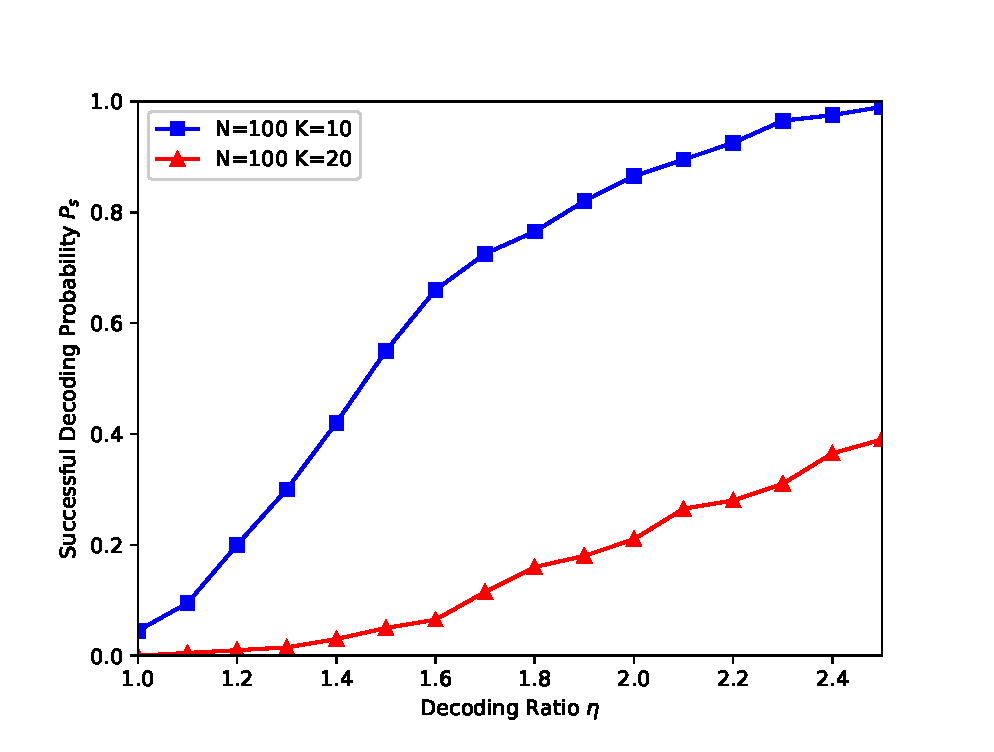
\includegraphics[width=0.9\columnwidth]{ratiovsprob.eps}
  \caption{Successfull decoding probability $P_s$ for different values of $N$, $K$ and decoding ratio $\nu$.}
  \label{fig:ratiovsprob}
\end{figure}

\section{Conclusions And Future Work}
\label{sec:conclusions}

\bibliographystyle{IEEEtran}
\bibliography{bibliography}

\end{document}
